\newpage
\renewcommand\thefigure{B.\arabic{figure}}    
\setcounter{figure}{0}

\renewcommand\thetable{A.\arabic{table}}    
\setcounter{table}{0}

\hypertarget{appendix}{%
\section*{Appendix}\label{appendix}}
\addcontentsline{toc}{section}{Appendix}

\hypertarget{a.-additional-tables}{%
\subsection*{A. Additional Tables}\label{a.-additional-tables}}
\addcontentsline{toc}{subsection}{A. Additional Tables}


\begin{table}[!h]
    \caption{Predicting response times with choices and conditions in Experiment 1}
    \vspace*{10pt}
    \centering

      \begin{tabular}{lll}
\hline
 & Intertemporal Choice & Count-the-Rabbits \\
\hline
Group & -0.684$^{***}$ & -0.792$^{***}$ \\
 & (0.141) & (0.144) \\
Question$\cdot1\{\text{Group}=0\}$ & -0.165 & 0.912$^{***}$ \\
 & (0.174) & (0.199) \\
Question$\cdot1\{\text{Group}=1\}$ & 0.457$^{***}$ & 0.849$^{***}$ \\
 & (0.101) & (0.132) \\
Choice & 0.954$^{*}$ & 1.291$^{***}$ \\
 & (0.399) & (0.456) \\
Choice$\times$Group & -0.762$^{*}$ & -1.265$^{***}$ \\
 & (0.304) & (0.229) \\
Choice$\times$Question$\cdot1\{\text{Group}=0\}$ & 0.001 & -0.138 \\
 & (0.257) & (0.23) \\
Choice$\times$Question$\cdot1\{\text{Group}=1\}$ & -0.12 & 0.263 \\
 & (0.195) & (0.175) \\\hline

observations & 4393 & 2179 \\
AIC & 18560.034 & 8711.872 \\
adj-$R^2$ & 0.381 & 0.55 \\
\hline
\end{tabular}
% INSERT reg_response_time

    \vspace*{4pt}
    \centering
    \begin{minipage}{0.85\textwidth}
    {\par\footnotesize Note: * $p<0.05$, ** $p<0.01$, *** $p<0.005$. Both models are estimated through 2SLS method. For first-stage regression, we use the model for Column (2) in Table \ref{tab:exp3_reg_intertemporal_choice} to predict intertemporal choices, and the model for Column (3) in Table \ref{tab:exp3_reg_rabbit_choice} to predict count-the-rabbits choices. The variable Choice which is 1 if the predicted choice is the sequence option and is 0 otherwise. For second-stage regression, indepdent variables are the predictors shown in the table plus task-specific dummies and their interactions with Choice, and participant-specific dummies. Standard errors (in the parentheses) are clustered at the subject level. $p$-values are calculated based on t-tests. }
    \end{minipage}
    \label{tab:exp3_reg_response_time}
\end{table}





\documentclass[12pt]{article}


\begin{document}
\begin{table}
    \caption{Regression results with risk-neutral utility function for Experiment 3}
    \vspace*{12pt}
    \centering

      \begin{tabular}{lllll}
\hline
 & \multicolumn{2}{r}{Front-end amount varies} & \multicolumn{2}{r}{Back-end amount varires} \\
 & (1) Pooled & (2) FE & (1) Pooled & (2) FE \\
\hline
$X_v$ & 0.181 & 0.316$^{***}$ & 0.139$^{***}$ & 0.318$^{***}$ \\
 & (0.339) & (0.044) & (0.011) & (0.03) \\
$X_v\cdot1\{M=M_{high}\}$ & 0.022$^{***}$ & 0.031$^{***}$ & 0.039$^{***}$ & 0.071$^{***}$ \\
 & (0.006) & (0.006) & (0.007) & (0.017) \\
$X_v\cdot1\{X_c=X_{mid}\}$ & -0.047 & -0.079$^{*}$ & -0.015 & -0.024 \\
 & (0.032) & (0.04) & (0.009) & (0.023) \\
$X_v\cdot1\{X_c=X_{high}\}$ & -0.083$^{**}$ & -0.135$^{***}$ & -0.026$^{**}$ & -0.031 \\
 & (0.031) & (0.041) & (0.01) & (0.023) \\
$X_v\cdot1\{T=T_{mid}\}$ & -0.033$^{***}$ & -0.058$^{***}$ &  &  \\
 & (0.006) & (0.012) &  &  \\
$X_v\cdot1\{T=T_{high}\}$ & -0.046$^{***}$ & -0.085$^{***}$ &  &  \\
 & (0.012) & (0.015) &  &  \\\hline

observations & 18840 & 18840 & 9420 & 9420 \\
AIC & 11455.38 & 6963.578 & 4215.293 & 2158.83 \\
\hline
\end{tabular}
% INSERT exp1_baseline_model

    \vspace*{4pt}
    \centering
    \begin{minipage}{0.85\textwidth}
    {\par\footnotesize Note: * $p<0.05$, ** $p<0.01$, *** $p<0.005$. Standard errors are clustered at the subject level and are reported in the parentheses. The $p$-values are calculated based on Wald tests. $X_c$ denotes the amount constant in a choice list, and its middle and highest levels are $X_{mid}$ and $X_{high}$. $T$ denotes the delay of the back-end amount, and its middle and highest levels are $T_{mid}$ and $T_{high}$. $M$ denotes amount in the single option, and its higher level is $M_{high}$. $X_v$ denotes the amount varying across rows. Every model includes question-specific dummies as random intercepts. Column (2) and (4) come from a model including participant-specific dummies as random intercepts.}
    \end{minipage}
    \label{tab:exp1_reg_baseline}
\end{table}

\end{document}




\documentclass[12pt]{article}


\begin{document}
\begin{table}
    \caption{Regression results on the censored data in Experiment 3}
    \vspace*{12pt}
    \centering

      \begin{tabular}{lllll}
\hline
 & \multicolumn{2}{r}{Front-end amount varies} & \multicolumn{2}{r}{Back-end amount varires} \\
 & (1) Pooled & (2) FE & (1) Pooled & (2) FE \\
\hline
$u(X_v)$ & 0.914$^{**}$ & 1.584$^{***}$ & 0.712$^{***}$ & 1.65$^{***}$ \\
 & (0.342) & (0.247) & (0.059) & (0.155) \\
$u(X_v)\cdot1\{M=M_{high}\}$ & 0.107$^{*}$ & 0.193$^{***}$ & 0.187$^{***}$ & 0.484$^{***}$ \\
 & (0.053) & (0.03) & (0.037) & (0.08) \\
$u(X_v)\cdot1\{X_c=X_{mid}\}$ & -0.314$^{*}$ & -0.499$^{*}$ & -0.134$^{***}$ & -0.281$^{*}$ \\
 & (0.129) & (0.226) & (0.047) & (0.111) \\
$u(X_v)\cdot1\{X_c=X_{high}\}$ & -0.509$^{***}$ & -0.828$^{***}$ & -0.248$^{***}$ & -0.5$^{***}$ \\
 & (0.127) & (0.231) & (0.048) & (0.111) \\
$u(X_v)\cdot1\{T=T_{mid}\}$ & -0.115$^{***}$ & -0.212$^{***}$ &  &  \\
 & (0.03) & (0.049) &  &  \\
$u(X_v)\cdot1\{T=T_{high}\}$ & -0.163$^{***}$ & -0.312$^{***}$ &  &  \\
 & (0.036) & (0.061) &  &  \\\hline

observations & 14915 & 14915 & 6594 & 6594 \\
AIC & 11226.482 & 6797.682 & 4120.484 & 2094.364 \\
\hline
\end{tabular}
% INSERT exp1_utility_censor

    \vspace*{4pt}
    \centering
    \begin{minipage}{0.9\textwidth}
    {\par\footnotesize Note: * $p<0.05$, ** $p<0.01$, *** $p<0.005$. FE denotes a model including participant-specific dummies as random intercepts. Each model and the estimation method are the same as Table \ref{tab:exp1_reg_utility}. However, for each question, the rows where all participants choose the same option are removed from the sample. }
    \end{minipage}
    \label{tab:exp1_reg_censor}
\end{table}

\end{document}



\newpage

\hypertarget{b.-additional-figures}{%
\subsection*{B. Additional Figures}\label{b.-additional-figures}}
\addcontentsline{toc}{subsection}{B. Additional Figures}

\begin{figure}
  \centering
  \begin{subfigure}{\textwidth}
    \centering
    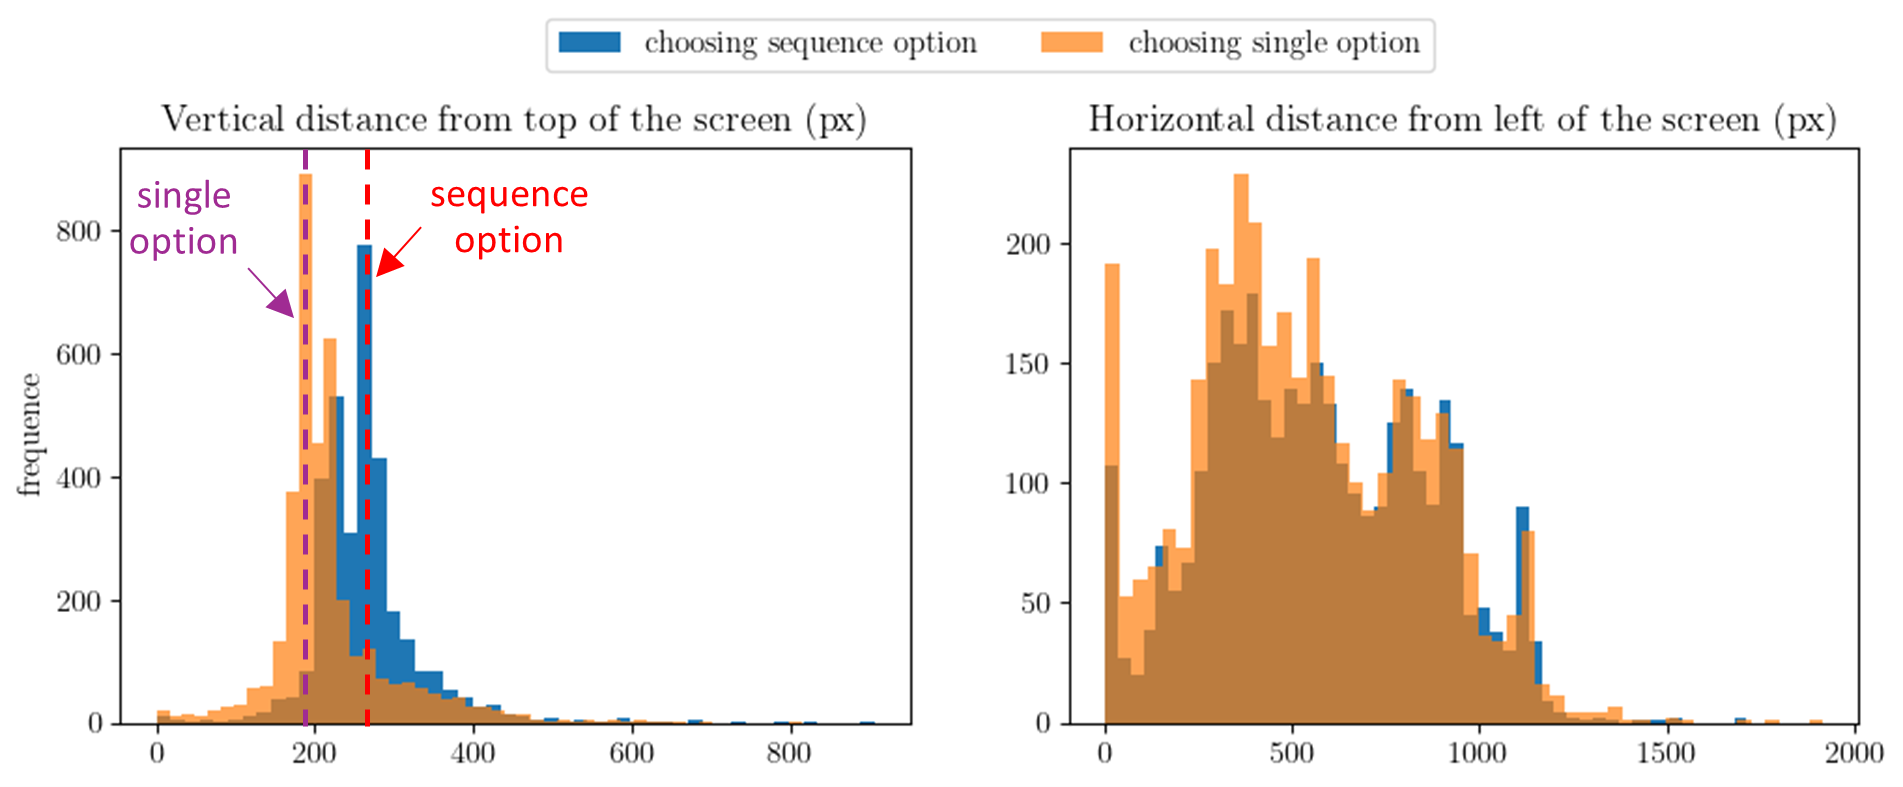
\includegraphics[width=\linewidth]{figures/exp3_mouse_intertemporal.png}
    \subcaption{Intertemporal Choice Task}
  \end{subfigure}
  \begin{subfigure}{\textwidth}
    \vspace{1.5em}
    \centering
    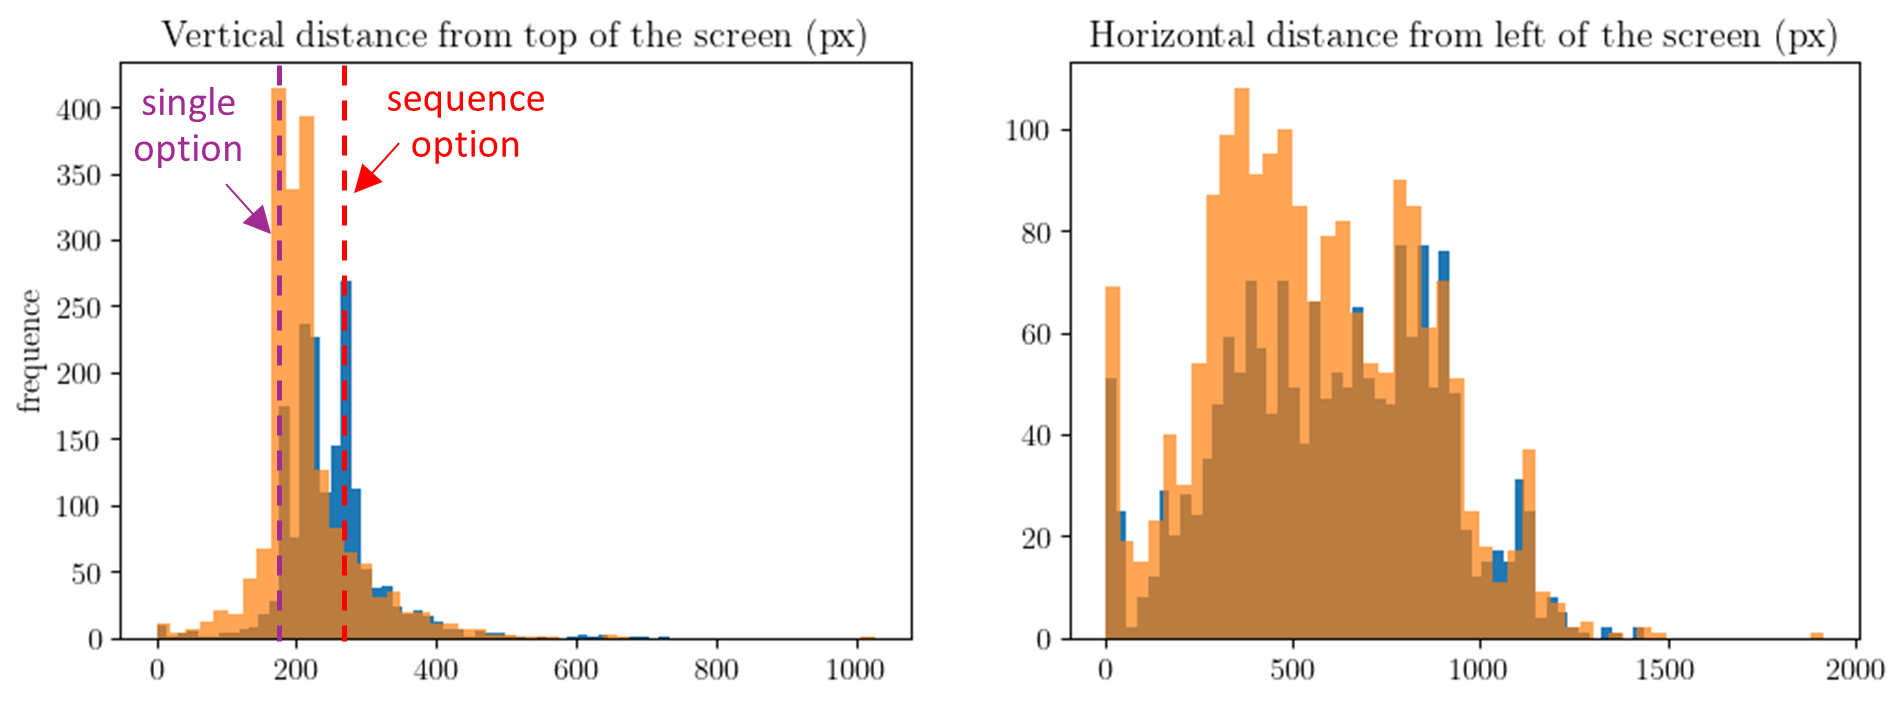
\includegraphics[width=\linewidth]{figures/exp3_mouse_rabbit.png}
    \subcaption{Count-the-Rabbits Task}
  \end{subfigure}
  \caption{Mouse positions recorded at the end of the forced viewing period}
  \label{fig:exp3_mouse_position}
\end{figure}

\begin{figure} 
\centering
\begin{subfigure}{0.85\textwidth}
  \hfill
  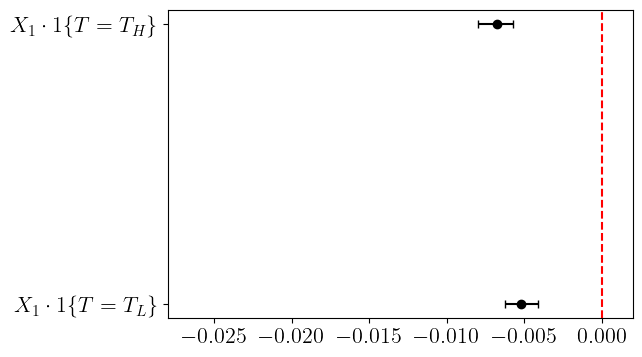
\includegraphics[width=0.85\linewidth]{figures/exp2_bootstrap_ci_baseline.png}
\end{subfigure}
\begin{subfigure}{0.85\textwidth} 
  \hfill
  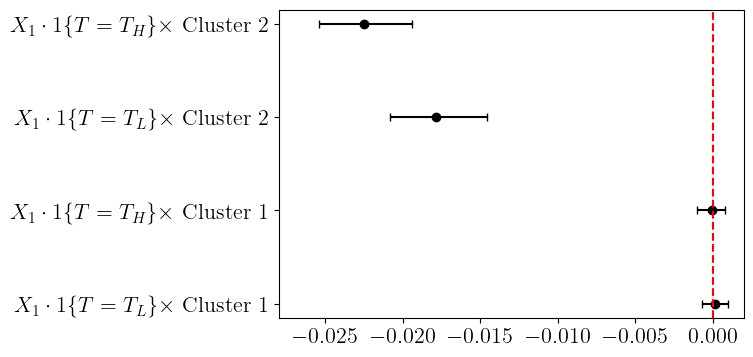
\includegraphics[width=\linewidth]{figures/exp2_bootstrap_ci_label.png} 
\end{subfigure}
\caption{Bootstrap 95\% confidence intervals for coefficients in the robust regressions}
\vspace*{4pt}
\centering

\begin{minipage}{1.0\textwidth}
{\par\footnotesize Note: The subfigures on the top and the bottom correspond to Column (5) and (6) in Table \ref{tab:exp2_seq_value_reg} respectively. The dots are the original estimates and the error bars indicate the confidence intervals. To approximate the distribution for each coefficient, we use the stratified bootstrap method. The observations are divided into three strata based on RLM results: the upper tail (with high residuals and a weight of 1), the lower tail (with low residuals and a weight of 1), and the others. We draw observations with replacement within each stratum and use them to estimate the coefficients. Each bootstrap sample is the same size as the original sample, and the process is repeated 1,000 times. }
\end{minipage}
\label{fig:exp2_bootstrap_ci}
\end{figure}

\begin{figure} 
\centering
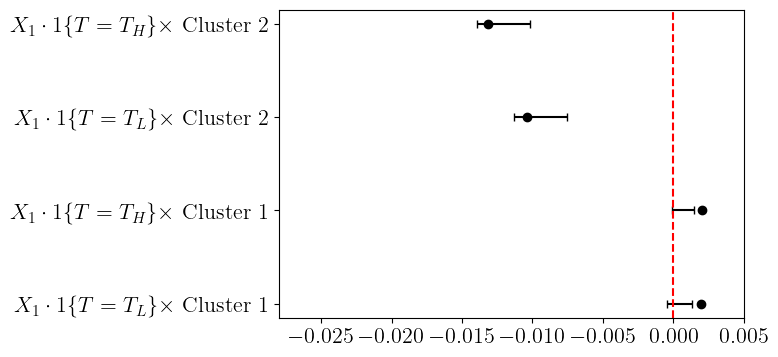
\includegraphics[width=0.85\linewidth]{figures/exp2_bootstrap_ci_label_gmm_fe.png}
\caption{Regression coefficients - using Gaussian mixture model for clustering}
\vspace*{4pt}
\centering

\begin{minipage}{1.0\textwidth}
{\par\footnotesize Note: The regression model is the same as Column (6) in Table \ref{tab:exp2_seq_value_reg}. Estimation method is the same as Figure \ref{fig:exp2_bootstrap_ci}. The dots are the original estimates and the error bars indicate the boostrap 95\% confidence intervals. }
\end{minipage}
\label{fig:exp2_bootstrap_ci_gmm}
\end{figure}

\newpage

\hypertarget{c.-method-to-estimate-risk-aversion-coefficient}{%
\subsection*{C. Method to estimate risk aversion
coefficient}\label{c.-method-to-estimate-risk-aversion-coefficient}}
\addcontentsline{toc}{subsection}{C. Method to estimate risk aversion
coefficient}

For any risky choice \(i\), let ``get \(X_i^R\) with a 50\% chance''
denote the risky option and ``get \(X_i^S\) with certainty'' denote the
safe option. Note \(X_i^R\) is constant within a choice list while
\(X_i^S\) is varying across rows. Assume that participants choose the
safe option with probability \(P_i^{\text{risk}}\), and\[
P_i^{\text{risk}} = \frac{1}{1+e^{-\frac{\Delta U}{\lambda}}}
\]where \(\Delta U = u(X_i^S) - 0.5\cdot u(X_i^R)\) and \(\lambda\)
(\(\lambda >0\)) is a temperature parameter that controls the randomness
of choice. The utility function is \(u(x)=(\omega+x)^\gamma\),
\(0<\gamma<1\), \(\omega\geq 0\). We fit the model with the maximum
likelihood method. The log-likelihood function is\[
LL(\gamma,\lambda) = \sum_{i=1}^N \xi_i\ln(P_i^{\text{risk}})+(1-\xi_i)\ln(1-P_i^{\text{risk}}) 
\]We use \(\gamma=1\), \(\lambda =1\) as the initial values and maximize
the log-likelihood function with the SLSQP algorithm. The model is
fitted on the 3,297 observations of the risky choices. In the solution,
\(LL=-1711.87\), \(\gamma=0.695\), \(\lambda=1.904\),
\(\omega\approx 2.245\times10^{-13}\).
